<<<<<<< HEAD
\section{Applikationslaget}
Applikationslaget er det lag af software i det samlede distribuerede system, som installeres eller afvikles hos brugeren. Applikationslaget er designet til at være platformuafhængigt, jf. systemets arkitektur. Derved er lagets model- og præsentationslag designet til at være portabelt, hvorimod view-laget er platformspecifikt. 
=======
% !TEX root = ../../../I4PRJ, Grp3 - Rapport.tex
\section{Applikationslaget}
Applikationslaget er det lag af software i det samlede distribuerede system, som installeres eller afvikles hos brugeren. Applikationslaget er designet til at være platformuafhængigt, jf. systemets arkitektur. Lagets model- og præsentationslag er designet til at være portabelt, hvorimod view-laget er platformspecifikt og designes seperat for hver platform. 
>>>>>>> 2e26db23f9227788585c53d38eecee7eacc75c56

Det overordnede design i applikationslaget illustreres ved sekvensdiagrammet i figur~\ref{fig:application_sd}. Her fremgår kommunikationsmønsteret mellem model-, view- og presenter-klasserne i applikationslagets design.

\begin{figure}
	\centering
	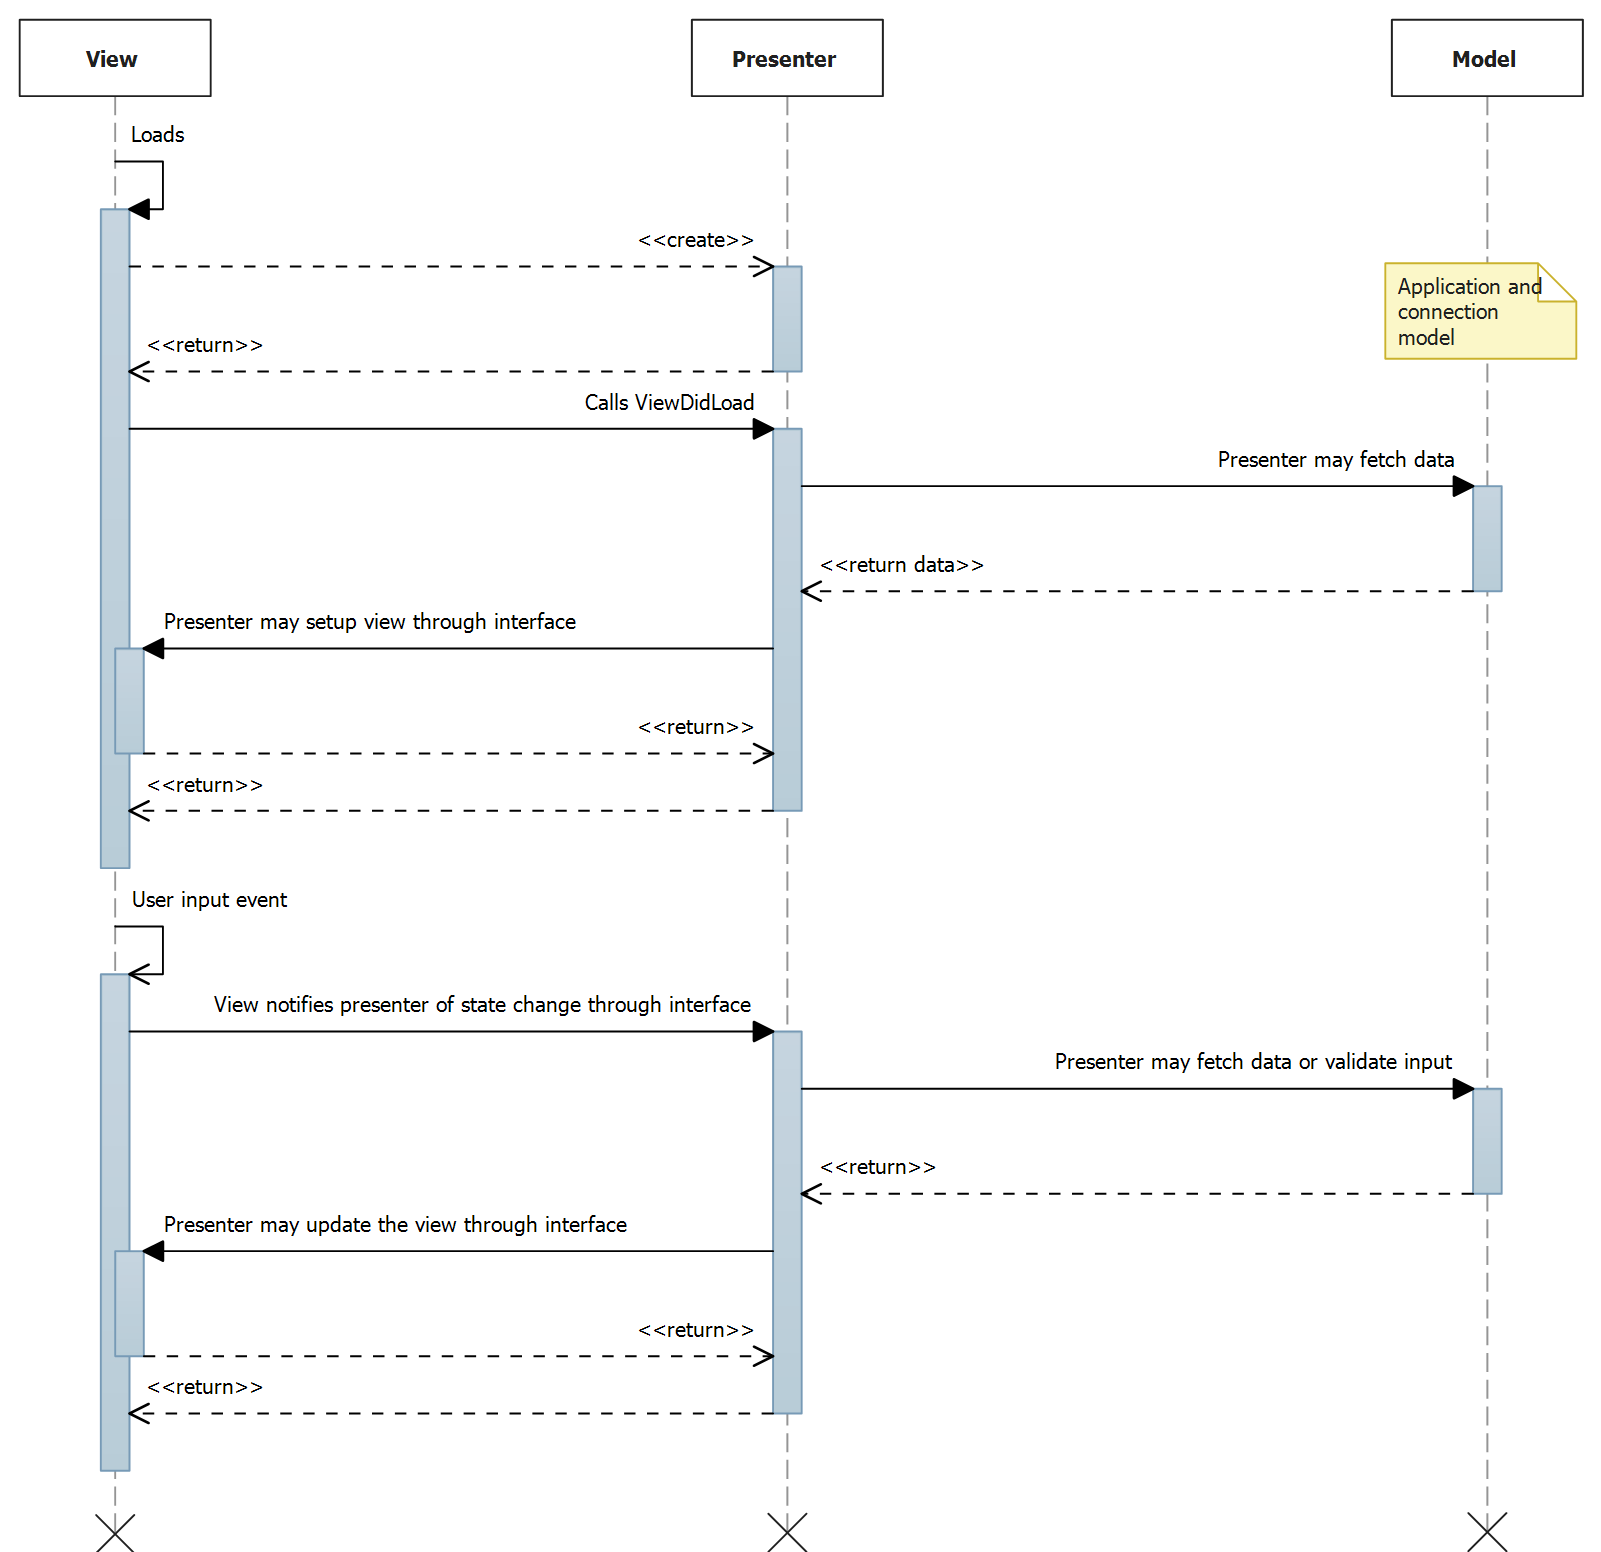
\includegraphics[width=1.0\linewidth]{figs/design/application_sd}
	\caption{Kommunikation i applikationslaget}
	\label{fig:application_sd}
\end{figure}

Som følge systemets multi-lag arkitektur kunne applikationslaget samt de platform-specifikke view-implementeringer
designes, uafhængigt af hinanden, så længe protokolbestemmende interfaces blev specificeret undervejs i processen. Interfaces for både presenters og views, er defineret ud fra de user stories, der har krævet deres design.

Præsentationslaget består af interfaces til presenters og views, samt konkrete presenters-klasser. View interfaces specificeres af de tilhørende presenter-klasser, og definerer presenter-klassens interaktion med view'et. På figur~\ref{fig:application_isignupview} ses klassediagrammet for ISignUpView-interfacet.

\begin{figure}
\centering
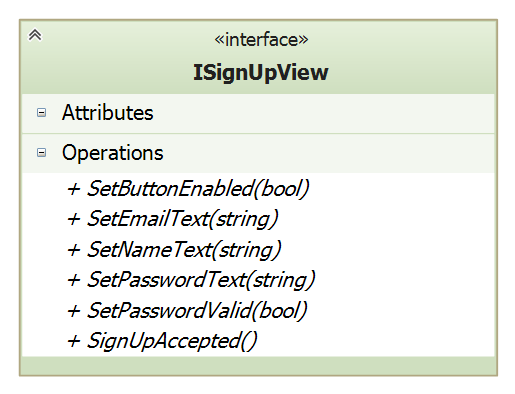
\includegraphics[width=0.35\linewidth]{figs/design/application_isignupview}
\caption{ISignUpView}
\label{fig:application_isignupview}
\end{figure}

Det konkrete signup view i hver platformspecifikke applikation implementerer view-interfacet og instantiere den tilhørende controller, hvis interface- og klassedesign ses på figur~\ref{fig:application_isignupviewcontroller}.

\begin{figure}
\centering
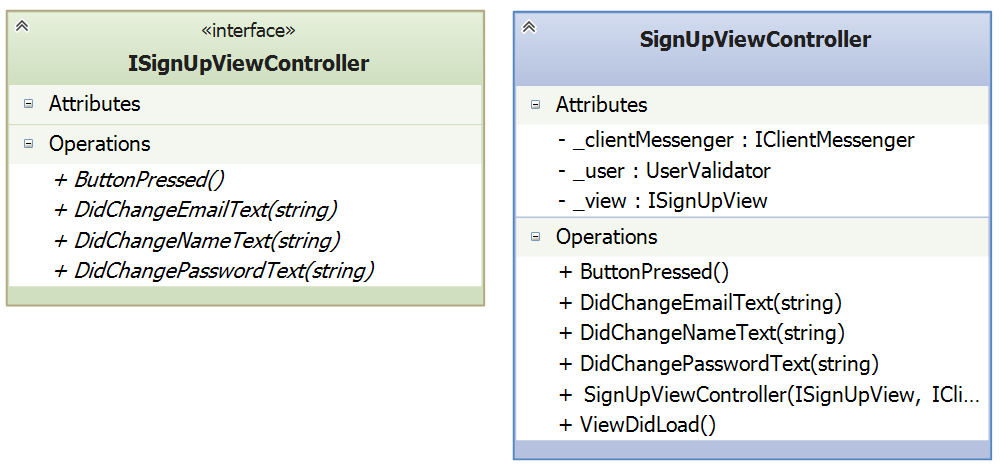
\includegraphics[width=0.7\linewidth]{figs/design/application_signupviewcontrollerandinterface}
\caption{ISignUpViewController og SignUpViewController}
\label{fig:application_isignupviewcontroller}
\end{figure}
Figur~\ref{fig:application_isignupviewcontroller} viser også, at den konkrete klasse indeholder flere metoder og attributter, som binder den konkrete klasse sammen med modellen. Modellen i applikationslaget består delvist af valideringslogik og klasser til kommunikation med resten af systemet. Det er attributter som \_clientMessenger, som er klienten, der kommunikerer med serveren og \_user af typen UserValidater, der validere om brugerinformationen er gyldig.

Den user story der omhandler visning af målinger, har ført til designet af følgende presenter-klasse.

\begin{figure}
\centering
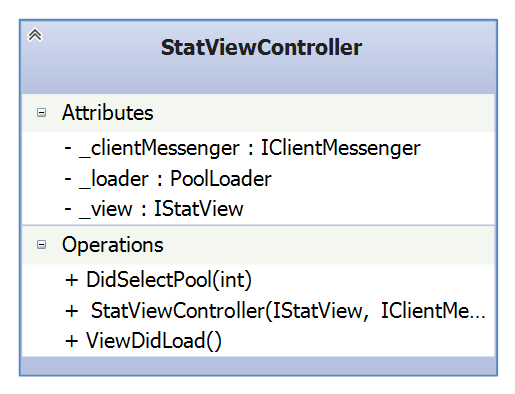
\includegraphics[width=0.35\linewidth]{figs/design/application_statviewcontroller}
\caption{StatViewController konkret klasse}
\label{fig:application_statviewcontroller}
\end{figure}

For yderligere forklaring se dokumentation afsnit Applikationslaget under Design.

\subsection{Windows GUI}
I Windows applikationen designes view-klasser, der implementerer view-interfacet defineret i præsentationslaget.
Designet af Windows GUI er lavet således, at codebehind filerne implementerer hver sit view-interfacet fra præsentationslaget. Codebehind agerer dermed som en bro, i mellem Smartpools præsentationslag, og WPF view-lag.

I klasse diagrammet nedenfor, ses Windows designet, af WinCreateUserView der implementerer ISignUpView fra applikationslaget og har en SignUpViewController.
\begin{figure}
\centering
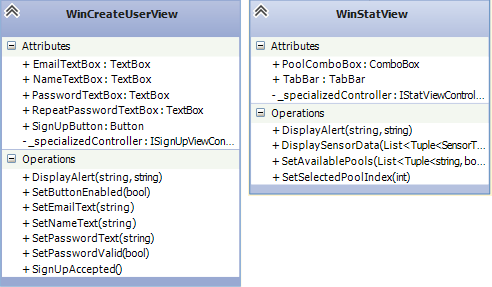
\includegraphics[width=0.7\linewidth]{figs/design/wincreateuserandwinstatviewview}
\caption{WinCreateUserView og WinStatView}
\label{fig:wincreateuserandwinstatviewview}
\end{figure}

Ligeledes er view klassen for WinStatView designet.
Klassen ses på figur~\ref{wincreateuserandwinstatviewview}.

For yderligere forklaring se dokumentation afsnit Applikationslaget under Design.